\documentclass[a4paper,12pt,numbered]{article}

\usepackage{soul}
\usepackage{amsmath}
\usepackage{mathtools}
\usepackage{amssymb,amsmath,amsfonts}
\usepackage[utf8]{inputenc}
\usepackage{graphicx}
\usepackage{geometry}
\usepackage{float}
\usepackage[german=quotes]{csquotes}
\usepackage{hyperref}
\usepackage{fancyhdr}
\usepackage{gensymb}
\usepackage{units}
\usepackage{hhline}
\usepackage{color}
\usepackage[export]{adjustbox}
\usepackage[nottoc,numbib]{tocbibind}
\usepackage[square,numbers]{natbib}
\usepackage{titling}
\usepackage{subfloat}
\usepackage{multicol}
\usepackage{caption}
\usepackage{authblk}
\usepackage{graphics}
\usepackage{subcaption}
\usepackage{pdfpages}

\iffalse
\title{}
\author[1]{Leon Buchholz}
\affil[1]{Humboldt Universität zu Berlin}
\date{08.02.2022}                     %% if you don't need date to appear
\setcounter{Maxaffil}{0}
\renewcommand\Affilfont{\itshape\small}
\fi


\geometry{a4paper, left=25mm, right=25mm, top=20mm, bottom=20mm}
\setlength\parindent{0pt}

\begin{document}

\newpage\null\thispagestyle{empty}\newpage

\iffalse
\maketitle
\fi

\section*{Abstract}
In this work, an investigation into using the inelasticity of inverse-beta-decay deep inelastic scattering neutrino events in the IceCube neutrino detector including DeepCore was conducted. It is shown that while the inelasticity can be used to statistically separate $\nu_\mu$ CC events in $\nu_\mu$/$\bar{\nu}_\mu$ CC events, the effect of this inelasticity separation on the sensitivity is not very significant. The sensitivity of the IceCube DeepCore detector towards the parameters $\Theta_{24},\Theta{34}$ of a sterile fourth neutrino are calculated and improved by changing to an improved sample and adding the inelasticity as an additional kinematic variable.
\newpage

\tableofcontents

\section{Introduction}

\section{Neutrinos}
\subsection{Neutrino Oscillation}

\section{Sterile Neutrinos}

In the Standard Model (SM) of particle physics, there are three known types, or ``flavors,'' of neutrinos: the electron neutrino ($\nu_e$), muon neutrino ($\nu_\mu$), and tau neutrino ($\nu_\tau$). These neutrinos are extremely light, electrically neutral particles that interact only via the weak force. Neutrino oscillations—where neutrinos change from one flavor to another—are a well-established phenomenon, implying that neutrinos have mass and that there is mixing between the neutrino flavor eigenstates and the neutrino mass eigenstates.

However, various experimental anomalies have hinted at the possible existence of a fourth type of neutrino, known as a \textbf{sterile neutrino}, which does not interact via the weak force and is only detectable through its mixing with the active neutrinos. The \textit{3+1 sterile neutrino model} introduces one sterile neutrino, $\nu_s$, in addition to the three active neutrinos, leading to a total of four mass eigenstates.


In the 3+1 model, the three active neutrinos ($\nu_e$, $\nu_\mu$, $\nu_\tau$) are supplemented by one sterile neutrino ($\nu_s$), which means that there are four mass eigenstates: $\nu_1$, $\nu_2$, $\nu_3$, and $\nu_4$. The mass of the sterile neutrino is generally assumed to be much larger than that of the active neutrinos. The relationship between flavor and mass eigenstates can be written as:


$\begin{pmatrix}
\nu_e \\
\nu_\mu \\
\nu_\tau \\
\nu_s
\end{pmatrix}
=
\bold{U}
\begin{pmatrix}
\nu_1 \\
\nu_2 \\
\nu_3 \\
\nu_4
\end{pmatrix}$,

where $\bold{U}$ is the extended $4 \times 4$ unitary mixing matrix. This matrix includes new mixing angles and phases that describe the interactions between the active and sterile neutrinos.


The motivation for sterile neutrinos comes from several experimental anomalies that are difficult to explain using only three active neutrinos. Some of the key anomalies include:
\begin{itemize}
    \item \textbf{Reactor neutrino anomaly:} Short-baseline neutrino experiments measuring reactor neutrino fluxes have detected a deficit of electron antineutrinos compared to theoretical predictions. This deficit could be explained by the oscillation of active neutrinos into sterile neutrinos.
    \item \textbf{LSND and MiniBooNE experiments:} These experiments observed unexpected oscillation patterns in short-baseline neutrino experiments, which cannot be easily accommodated by the standard three-neutrino oscillation model.
\end{itemize}

These anomalies suggest the possible existence of a sterile neutrino with a mass on the order of 1 eV, which would mix with the active neutrinos and modify the oscillation probabilities observed in experiments.


The inclusion of a sterile neutrino in the 3+1 model introduces additional parameters, such as:
\begin{itemize}
    \item Three new mixing angles: $\theta_{14}$, $\theta_{24}$, and $\theta_{34}$, which describe the mixing between the sterile and active neutrinos.
    \item One new mass-squared difference, $\Delta m_{41}^2 = m_4^2 - m_1^2$, which describes the mass splitting between the sterile neutrino and the light active neutrinos.
\end{itemize}

These additional parameters modify the neutrino oscillation probabilities. For example, the survival probability of an electron neutrino, $P(\nu_e \rightarrow \nu_e)$, in a short-baseline experiment is given by:
\[
P(\nu_e \rightarrow \nu_e) = 1 - 4 |U_{e4}|^2 (1 - |U_{e4}|^2) \sin^2 \left( \frac{\Delta m_{41}^2 L}{4E} \right),
\]
where $L$ is the baseline (distance between source and detector) and $E$ is the neutrino energy.


The 3+1 sterile neutrino model offers a possible explanation for several experimental anomalies that cannot be explained by the Standard Model alone. Although there is no direct detection of sterile neutrinos yet, ongoing and future experiments will continue to test this hypothesis. The discovery of a sterile neutrino would have profound implications for both particle physics and cosmology, potentially reshaping our understanding of the universe and the fundamental properties of neutrinos.

\subsection{Source of atmospheric neutrinos}

Atmospheric neutrinos are produced when cosmic rays, which are high-energy particles primarily composed of protons and atomic nuclei, collide with molecules in Earth's upper atmosphere. When these cosmic rays, typically from outside the solar system, strike nitrogen or oxygen nuclei in the atmosphere, they initiate a cascade of secondary particles, known as an air shower.

In this shower, mesons such as pions (\(\pi^\pm\)) and kaons (\(K^\pm\)) are produced. These unstable particles quickly decay into lighter particles, including muons (\(\mu^\pm\)) and muon neutrinos (\(\nu_\mu\)):

\[
\pi^+ \rightarrow \mu^+ + \nu_\mu \quad \text{and} \quad \mu^+ \rightarrow e^+ + \nu_e + \bar{\nu}_\mu
\]

Similarly, negative pions decay into anti-muon neutrinos (\(\bar{\nu}_\mu\)) and electrons. These decays result in a flux of neutrinos in the atmosphere, predominantly muon neutrinos and electron neutrinos.

\section{The IceCube Neutrino Observatory}
The \textbf{IceCube Neutrino Observatory} is a cutting-edge research facility located at the South Pole, designed to detect neutrinos—tiny, nearly massless particles that rarely interact with matter. Spanning a cubic kilometer of ice, IceCube uses a vast array of light detectors buried deep beneath the Antarctic ice to capture the faint flashes of light, known as Cherenkov radiation, produced when neutrinos collide with ice particles. The main goal of IceCube is to study high-energy neutrinos originating from cosmic events, such as supernovae, gamma-ray bursts, or black holes, which may help unravel the mysteries of the universe.

IceCube consists of 86 strings, each holding 60 digital optical modules (DOMs) spread out between 1,450 to 2,450 meters below the ice surface. These DOMs detect the Cherenkov light from neutrino interactions and allow scientists to reconstruct the direction, energy, and type of neutrinos that pass through the detector. IceCube has made significant contributions to astrophysics, including detecting the first-ever high-energy neutrino in 2013 linked to a known astrophysical source, a blazar.

\subsection*{DeepCore}

A key component of the IceCube detector is \textbf{DeepCore}, a densely instrumented subarray located within the bottom center of IceCube. While IceCube primarily focuses on high-energy neutrinos (above TeV energies), DeepCore is optimized for lower-energy neutrinos in the GeV range, making it highly sensitive to atmospheric neutrinos and neutrinos from other potential sources like dark matter annihilations or supernovae.

DeepCore consists of 8 additional strings with DOMs placed more closely together, between depths of 2,100 to 2,450 meters. This denser arrangement, along with the extremely clear ice at these depths, allows DeepCore to detect lower-energy neutrinos with greater precision than the rest of IceCube. The presence of DeepCore enables IceCube to study a broader spectrum of neutrino energies and provides opportunities for probing fundamental questions in particle physics, such as neutrino oscillations and the search for new physics beyond the Standard Model.

\subsection{Events in the IceCube detector}

In the IceCube Neutrino Observatory, neutrinos interact with matter in the ice, producing secondary charged particles like muons and electrons. These particles, when moving faster than the speed of light in ice, emit Cherenkov radiation, which is detected by IceCube's optical sensors (photomultiplier tubes).

Muon events: When a neutrino produces a muon in the ice, the muon travels over long distances, creating a "track" of Cherenkov light. These tracks are relatively straight and extended, allowing for precise determination of the direction of the incoming neutrino. Muons are often produced in charged-current interactions of muon neutrinos and are key for identifying high-energy neutrinos.

Electron and tau events (cascades): Electrons and taus, on the other hand, generate "cascade" events. In these cases, when an electron neutrino interacts with matter, the resulting electron induces an electromagnetic shower, and tau neutrinos can produce hadronic or electromagnetic showers depending on how the tau decays. These cascades are more localized, producing a spherical or blob-like light pattern. Cascades allow for good energy reconstruction but have lower directional accuracy compared to muon tracks.

Thus, the event topology in IceCube depends on the type of neutrino interaction, with muons producing elongated track-like signatures and electrons or tau decays forming compact cascade-like events.

\section{Event Simulation}

\section{Data Processing}

\section{Final Analysis Binning}

\subsection{Inelasticity in inverse beta decay in the IceCube detector}

Inelasticity plays a crucial role in the analysis of \(\nu_\mu\) charged-current (CC) interactions in the IceCube detector. In these interactions, a muon neutrino (\(\nu_\mu\)) interacts with a nucleon, typically a proton or neutron, producing a muon (\(\mu\)) and a hadronic shower:

\[
\nu_\mu + N \rightarrow \mu + X
\]

Here, \(X\) represents the hadronic products from the interaction. The inelasticity, denoted by \(y\), quantifies the fraction of the incoming neutrino's energy that goes into the hadronic shower rather than the muon. It is expressed as:

\[
y = 1 - \frac{E_\mu}{E_{\nu_\mu}}
\]

where \(E_\mu\) is the energy of the outgoing muon, and \(E_{\nu_\mu}\) is the total energy of the incident muon neutrino. A lower inelasticity implies that most of the neutrino's energy is transferred to the muon, producing a long, well-defined muon track in the detector. Conversely, a higher inelasticity means that more energy is deposited in the hadronic shower, resulting in a more localized cascade-like signal in addition to the muon track.

In IceCube, these events are particularly valuable as muon tracks provide excellent directional information, while the energy distribution between the muon and the hadronic shower gives insight into the inelasticity of the interaction. Accurate reconstruction of inelasticity is critical for determining the energy of the original neutrino and understanding its interaction properties.

Since the earth consists of neutrons, protons and electrons, the scattering of the respective neutrino types are not expected to produce identical inelasticity distributions. The central goal of this work therefore is to use the expected difference in the inelasticity distributions of $\nu_\mu$ CC and $\bar{\nu}_\mu$ CC to separate neutrinos and anti-neutrinos to boost the sensitvity towards relevant oscillation parameters of sterile neutrinos.

\section{IceCube FLERCNN Event Selection}
\section{Oscillograms}

In order to separate the types of muon-neutrinos, it is necessary to understand the impact of the inherent parameters of the sterile neutrino towards this separation. In this analysis only the parameters $\Theta_{24},\Theta_{34}$ and later the CP-violating phase $\delta_{24}$ are investigated.


\subsection{Sterile Model}
\section{Inelastictiy Reconstruction}

For this analysis multiple reconstructions of the inelasticity for simulated Monte-Carlo (MC) neutrino events in the IceCube detector corresponding to 9.28 years worth of data were investigated and used. 
Multiple inelasticity reconstructions were provided and investigated for their performance. Of the five provided reconstructions, four were done by convolutional-neural-networks (CNNs) that differed in the training datasets that were used, while the other reconstruction was performed by a boosted-decision tree (BDT).
\\
In the case of the CNN-based reconstructions, both $\nu_\mu-cc, \bar{\nu}_\mu-cc$ events were used in the training datasets while the BDT-based reconstruction was optimized using a pure $\nu_\mu-cc$ event dataset.
\\ \\
The CNNs differ in the datasets they were trained on. Two CNN-based reconstructions were each trained on IceCube data that underwent up to level 3 and respectively level 6 of the IceCube event selection. Of those reconstructions trained on the same level, one used only neutrino events having a primary neutrino energy of at least 5 GeV with the other having a higher minimum threshold of 30 GeV for the data used in training.

\subsection{Reconstruction Performance}
\subsubsection{CNN-based Reconstructions}

As there are multiple CNN-based reconstructions it is of interest to investigate the impact of the different training sets on the reconstruction performance. In the following section the reconstructions will be investigated for their performance in various regions of energy. Only the $\nu_\mu-cc, \bar{\nu}_\mu-cc$ channels are of interest as every other channel shows poor reconstruction performance. This is not only due to the underlying training of the samples but also the event topology discussed before, as muons leave much cleaner signals that are easier to reconstruct than electron or tauons. To avoid overly long descriptions, the reconstructions will be referred to by the key differences in their training, e.g. the 30 GeV reconstruction referring to the CNN-based reconstruction trained on neutrino events with a minimum true energy threshold of 30 GeV.

\newpage

\begin{figure}[H]
\centering
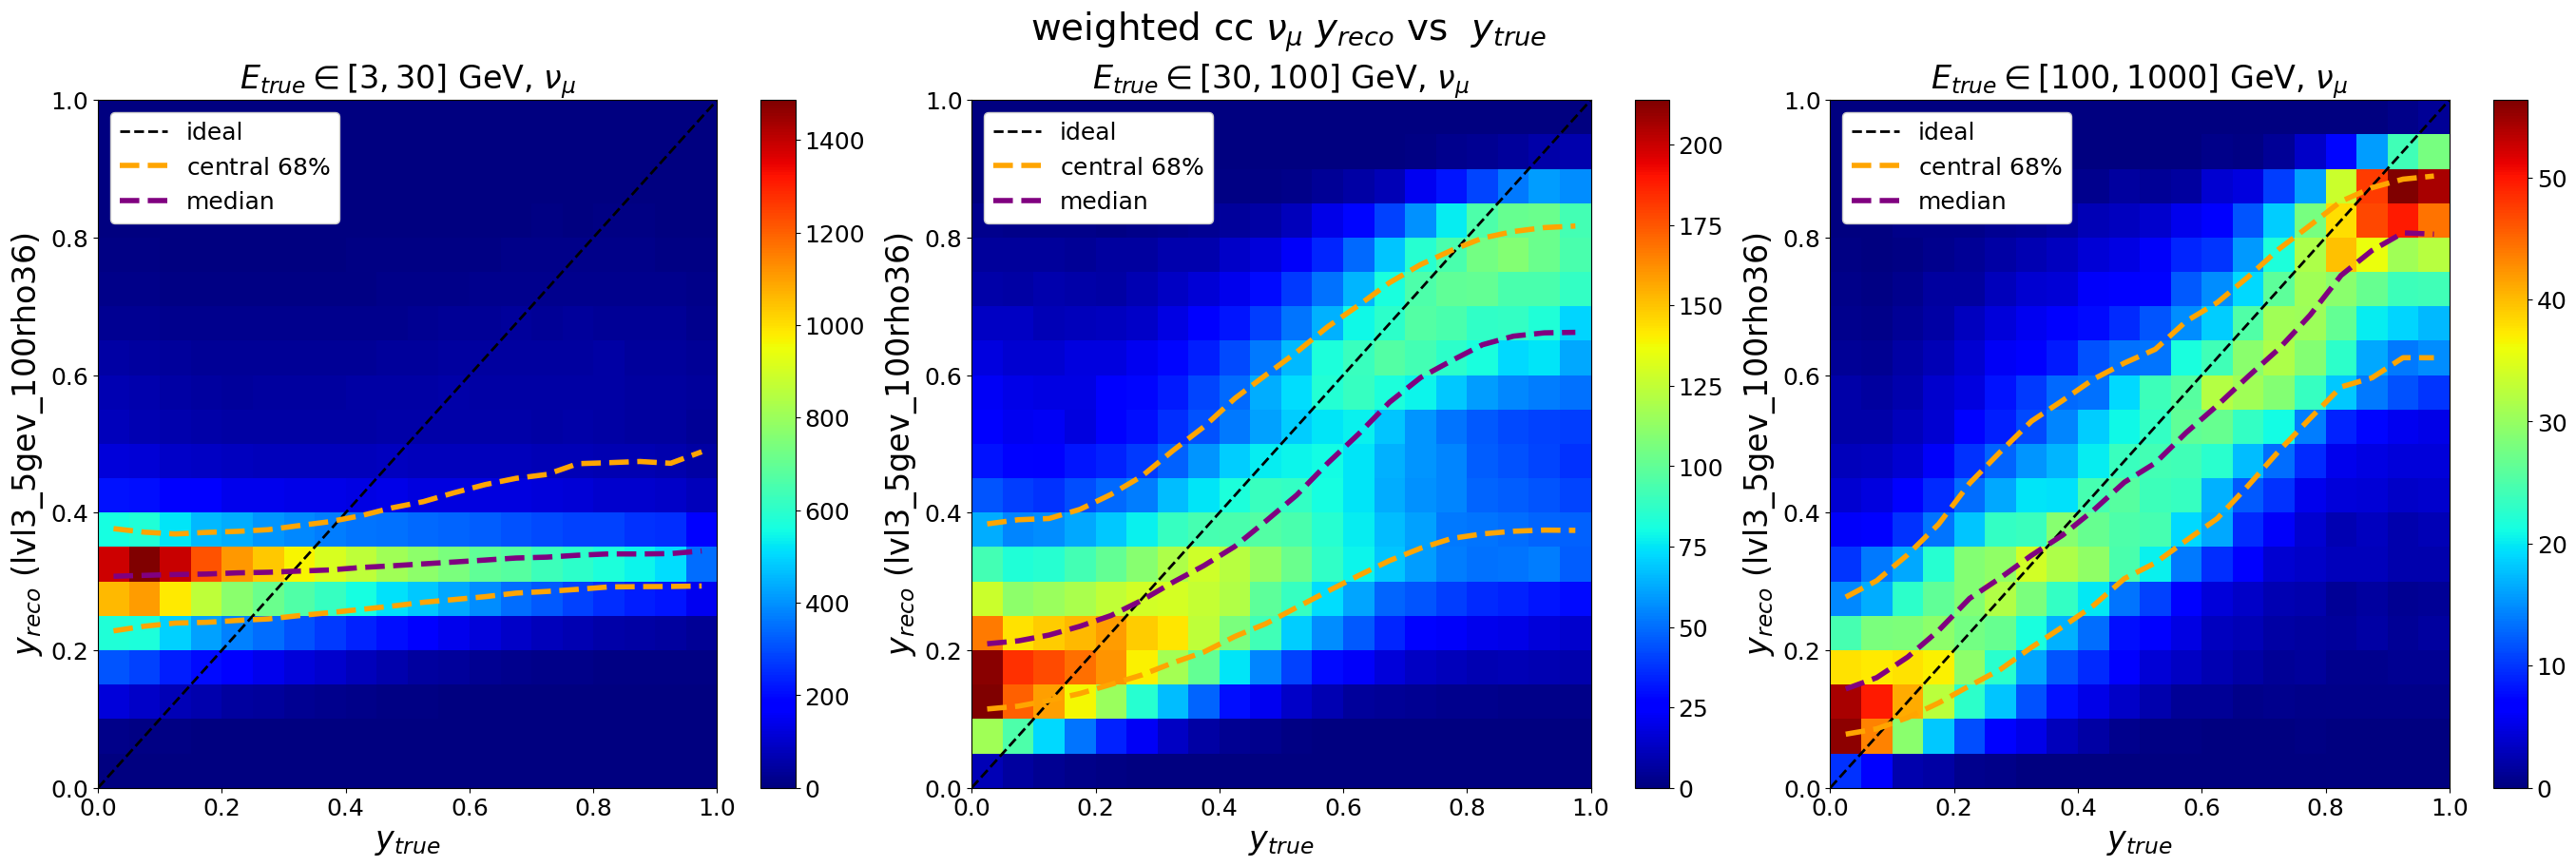
\includegraphics[width=\textwidth]{Graphics/Inelasticity/WithCentral68/weighted/weighted_cc_ytruevsyreco_lvl3_5gev_100rho36_numu.png}
\caption{A}
\end{figure}

\begin{figure}[H]
\centering
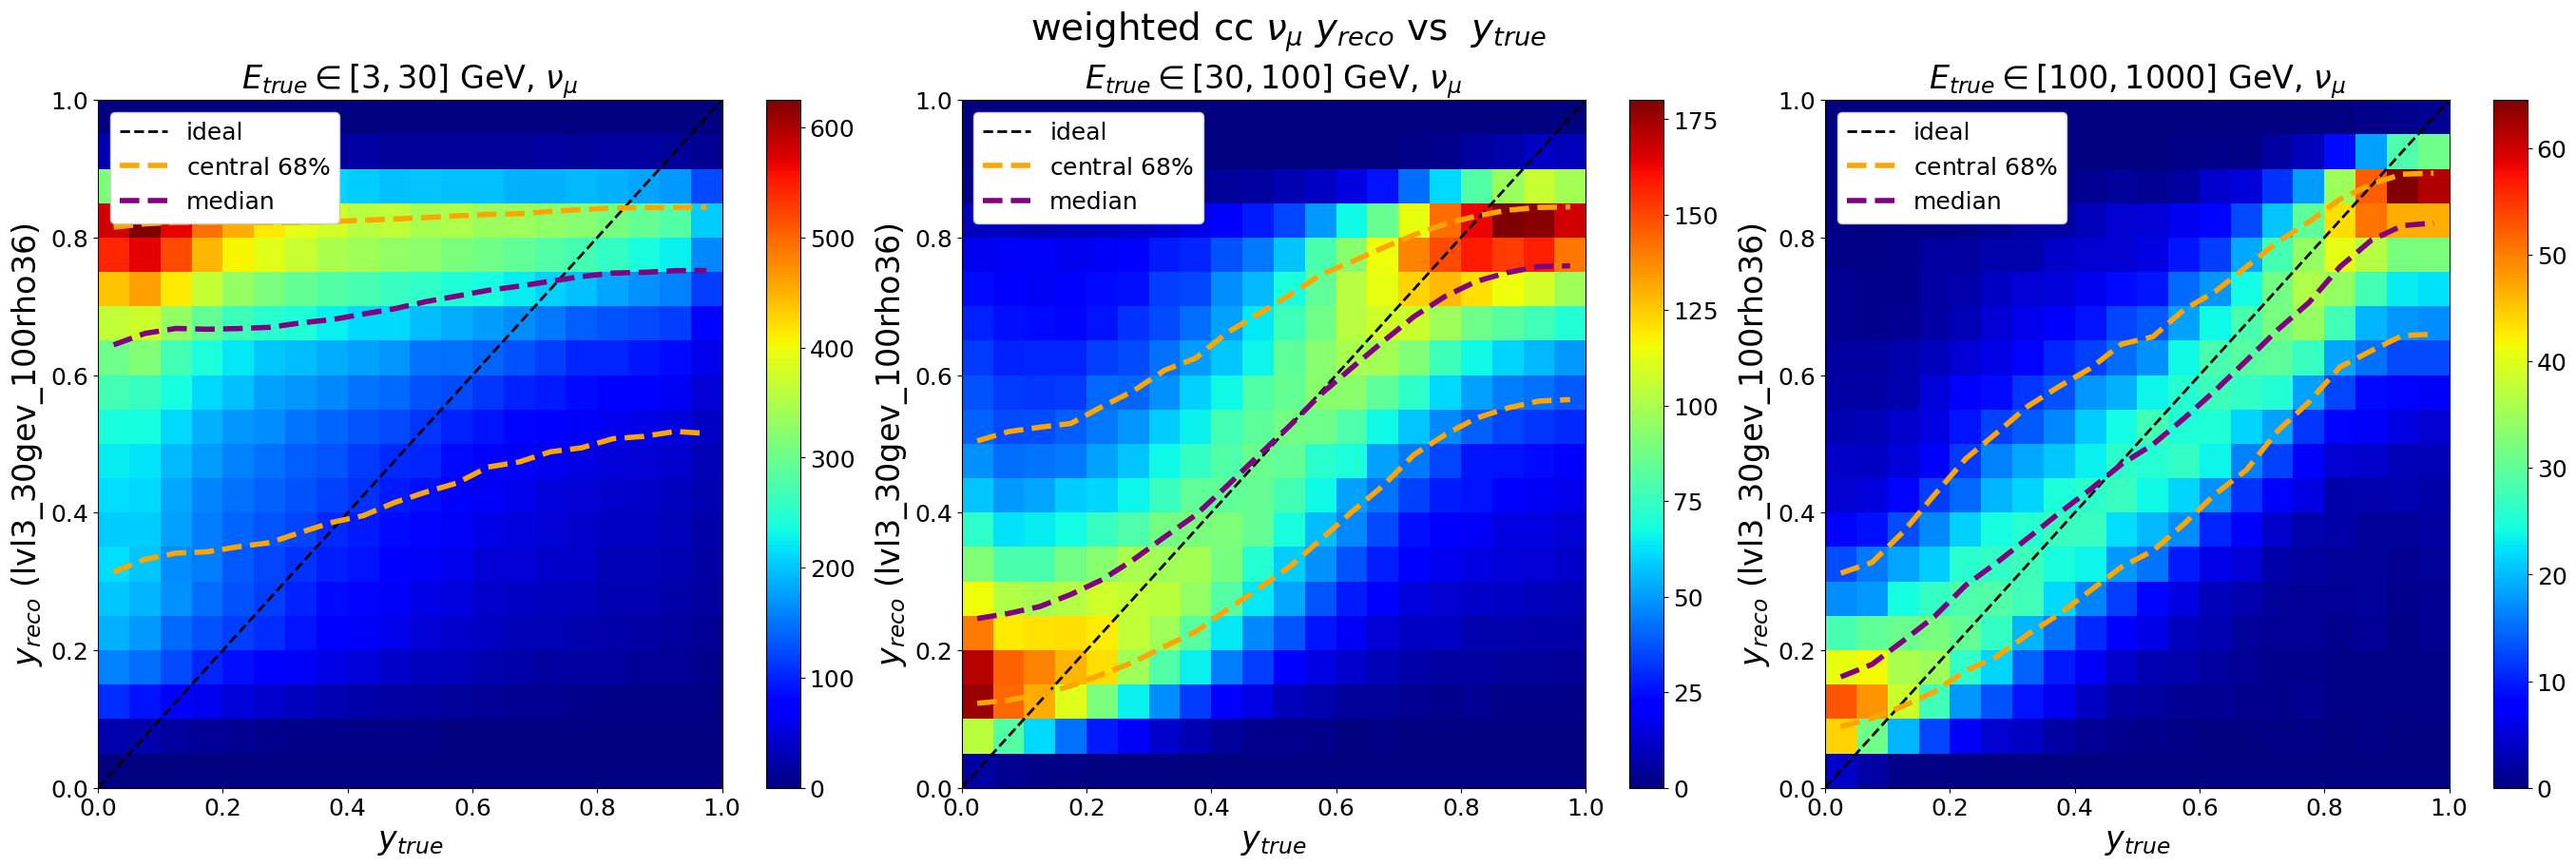
\includegraphics[width=\textwidth]{Graphics/Inelasticity/WithCentral68/weighted/weighted_cc_ytruevsyreco_lvl3_30gev_100rho36_numu.png}
\caption{B}
\end{figure}

The higher minimum energy threshold for the CNN trained on neutrino events with an energy at least 30 GeV allows a better reconstruction at higher inelasticities in all cases. However, the higher minimum energy threshold also increases the median reconstructed inelasticity for lower values of the true inelasticity and events above 30 GeV. Besides that, the poor performance of the inelasticity reconstruction for events with low energy is also clearly visible with neither the "5 GeV" nor the "30 GeV" trained CNN-based reconstructions providing satisfactory reconstruction performance. These effects are likely caused by the inherent energy distribution as events with big inelasticity and small energy are less likely to occur due to the majority of the four momentum in the scattering staying with the primary particle (muon/antimuon). While there are typically more events in the low inelasticity region, the additionally overall more consistent performance of the 30 GeV reconstruction in the [30,100] GeV bin is evaluated to be the better choice.

\begin{figure}[H]
\centering
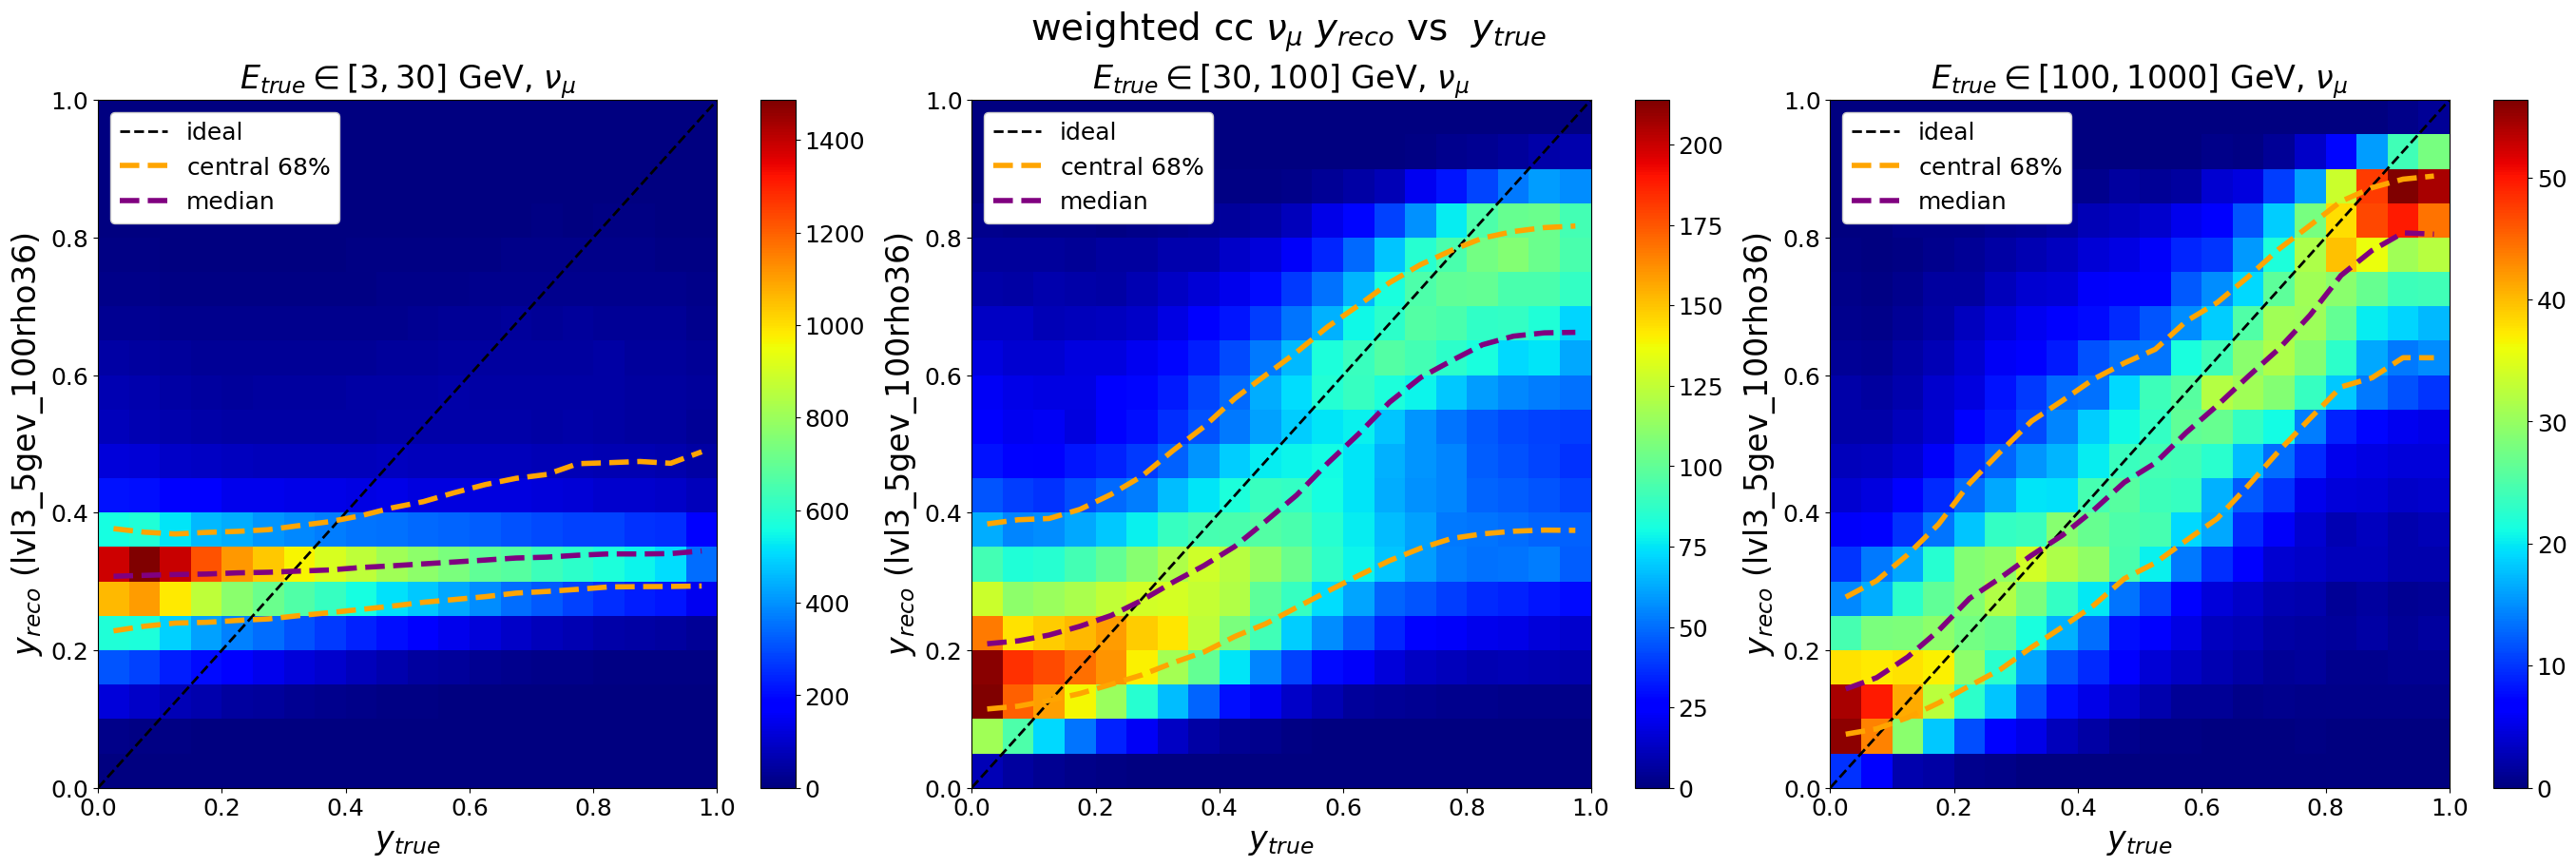
\includegraphics[width=\textwidth]{Graphics/Inelasticity/WithCentral68/weighted/weighted_cc_ytruevsyreco_lvl3_5gev_100rho36_numu.png}
\caption{A}
\end{figure}

\begin{figure}[H]
\centering
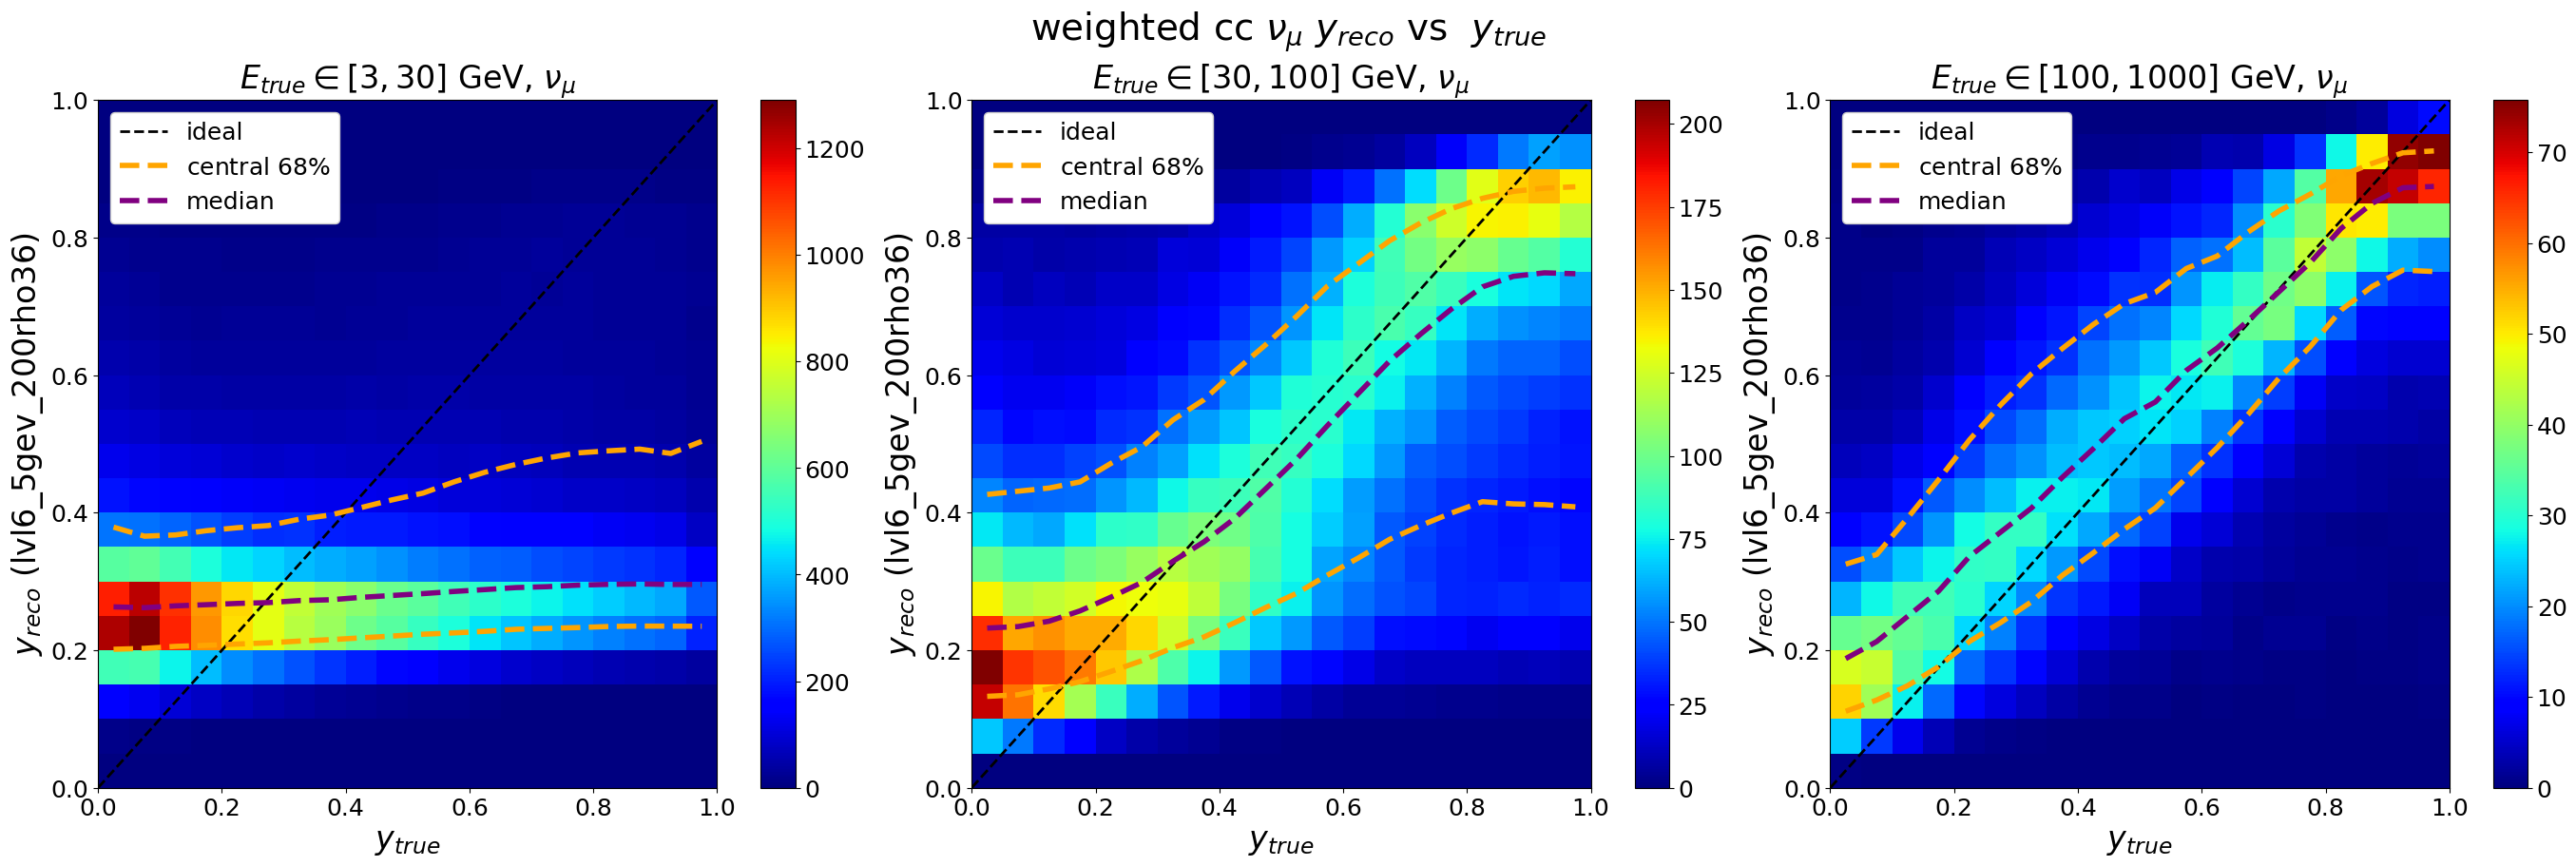
\includegraphics[width=\textwidth]{Graphics/Inelasticity/WithCentral68/weighted/weighted_cc_ytruevsyreco_lvl6_5gev_200rho36_numu.png}
\caption{B}
\end{figure}

Above figure shows the respective performance of the CNN-based inelasticity reconstruction trained on level 3 and level 6 data and the respective vertex regions. The level 6 reconstruction shows better performance at higher inelasticities and a more consistent reconstruction in the medium energy region. However, it has worse performance at low inelasticities and at low energy. After weighing the tradeoffs, the CNN trained on level 6 data with neutrino energy of at least 30 GeV is evaluated to be the slightly better choice.

\subsubsection{BDT-based Reconstruction}

As the BDT-based inelasticity reconstruction was only optimized for the $\nu_\mu-cc$ channel it is necessary to check the reconstruction performance for both types of neutrinos.

\begin{figure}[H]
\centering
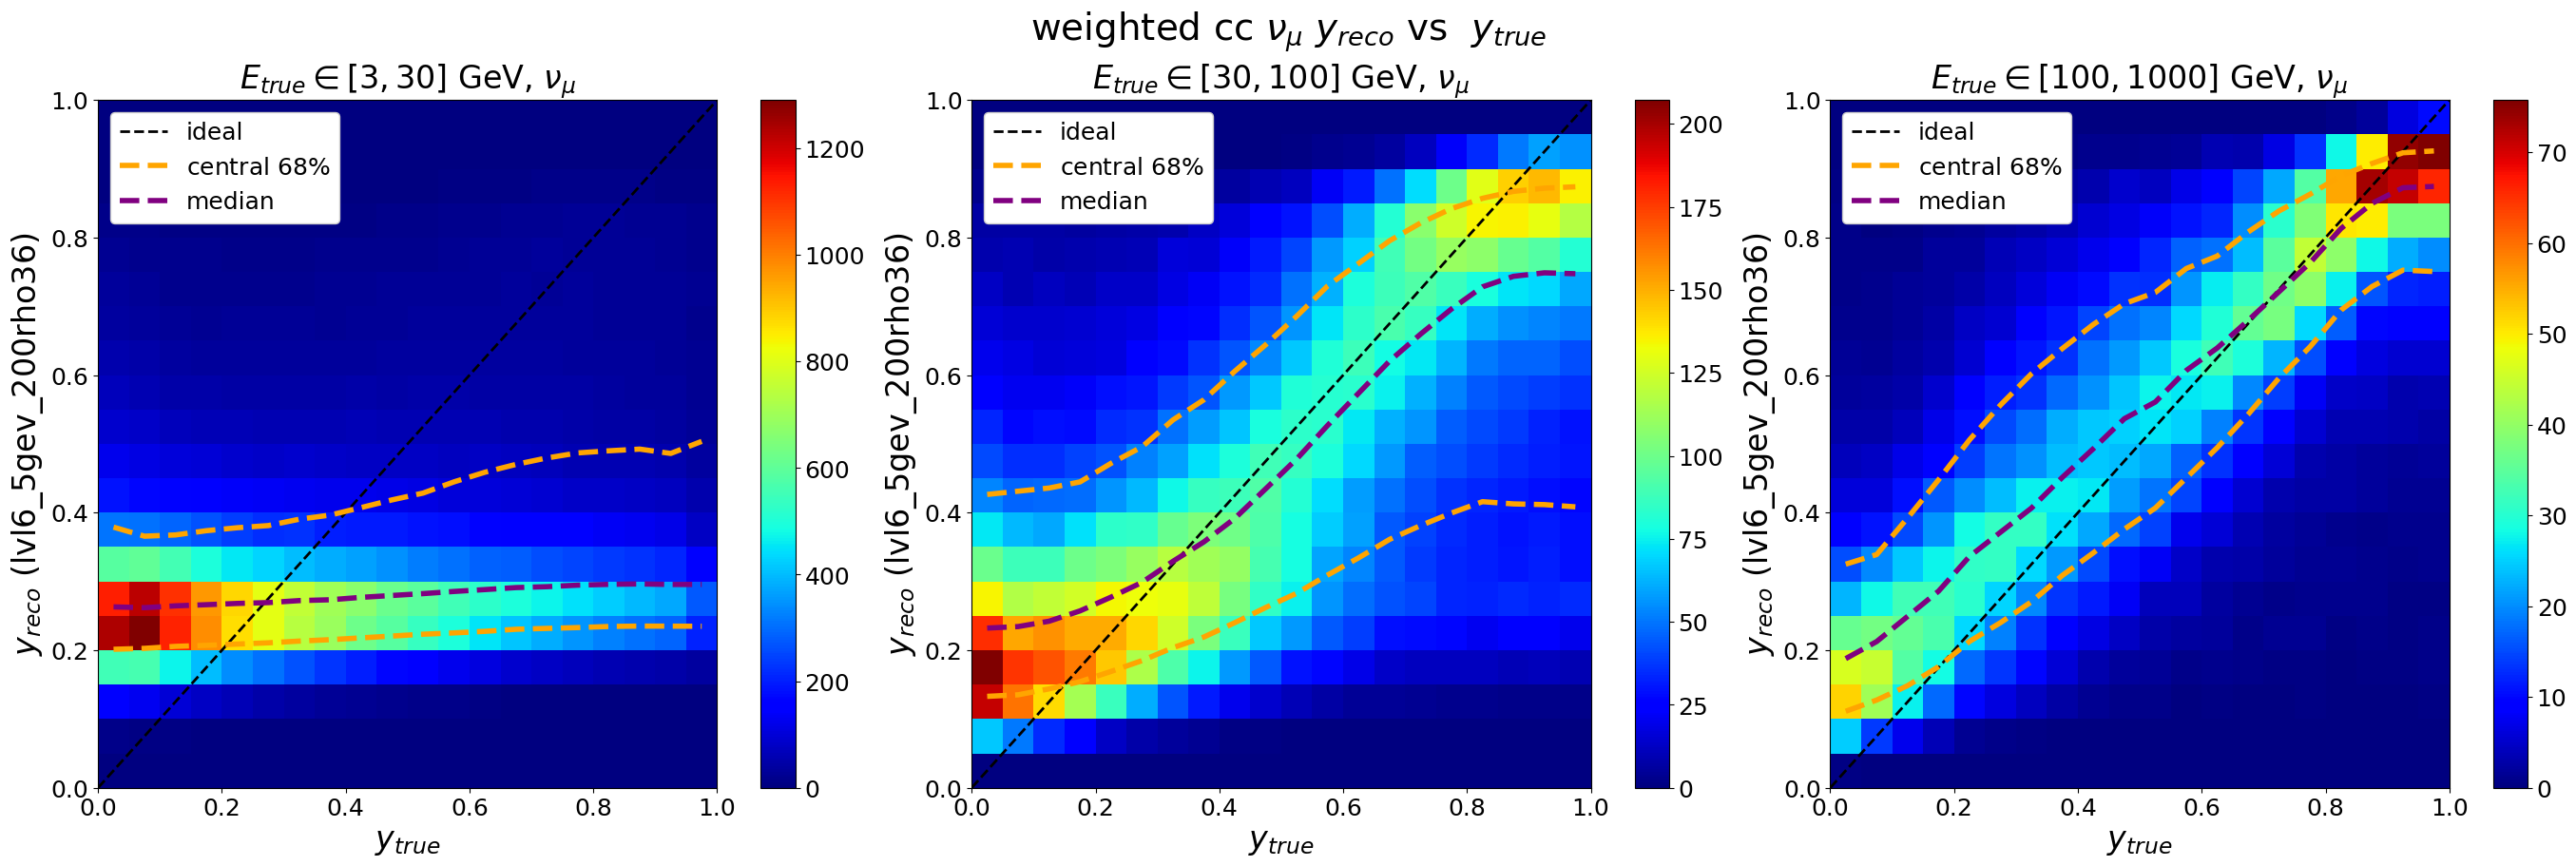
\includegraphics[width=\textwidth]{Graphics/Inelasticity/WithCentral68/weighted/weighted_cc_ytruevsyreco_lvl6_5gev_200rho36_numu.png}
\caption{B}
\end{figure}

As is evident from the above show reconstruction performance of the BDT-based method, there are no noticable issues inherent from the training with the reconstruction performance being similar to the CNN-based methods. In the following part, the difference of the reconstructed to the true inelasticity (resolution) will be compared between the facored CNN-based reconstruction and the BDT-based one.

\begin{figure}[H]
\centering
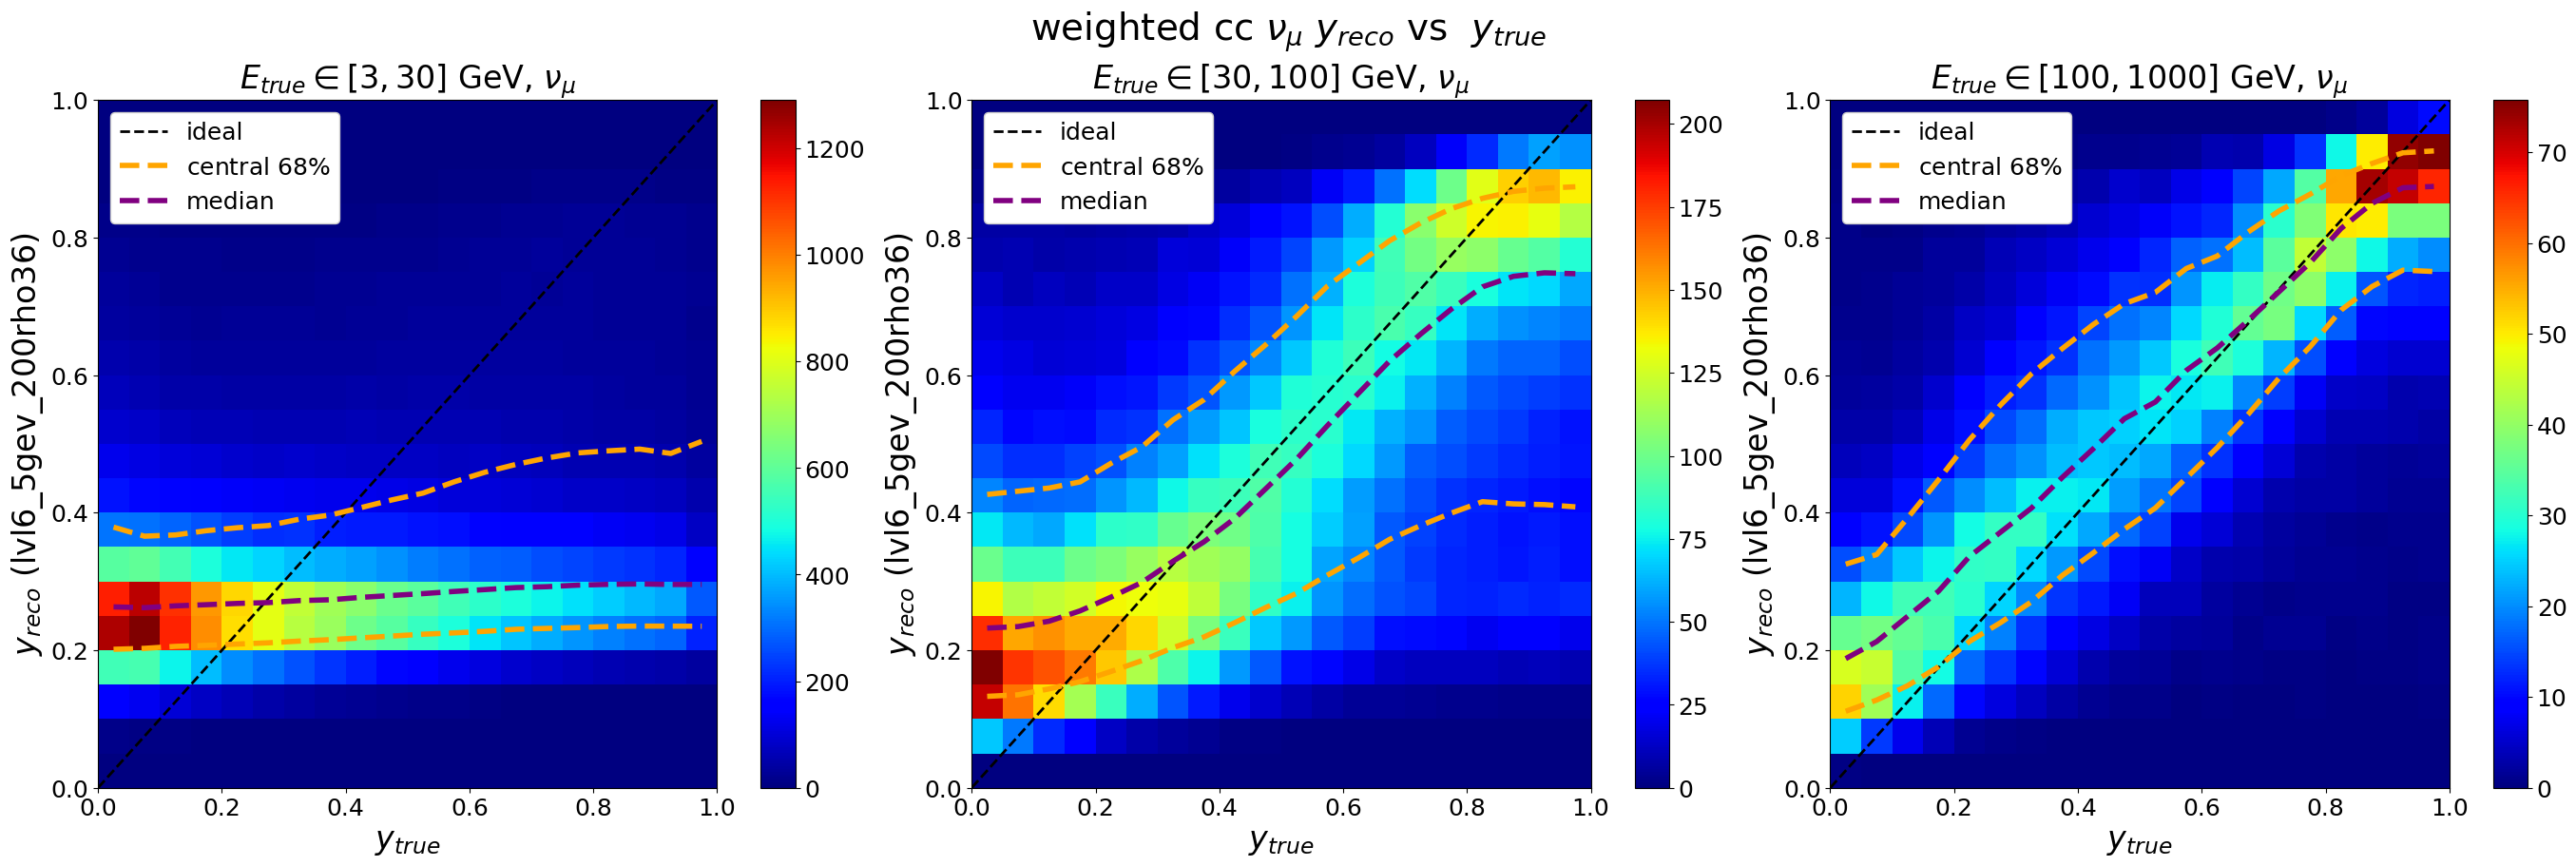
\includegraphics[width=\textwidth]{Graphics/Inelasticity/WithCentral68/weighted/weighted_cc_ytruevsyreco_lvl6_5gev_200rho36_numu.png}
\caption{B}
\end{figure}

The BDT-based reconstruction shows better performance for both types of muon-neutrinos and across the board with also deteriorating performance for lower energy. As such the analysis will be conducted with the BDT-based reconstruction and in the remaining part of the analysis, the inelasticity reconstruction will refer to the BDT-based one by default unless specifically mentioned.

\subsection{Inelasticity PID Correlation}

As only $\nu_\mu$ CC events have a usable inelasticity reconstruction, likely due to their physical topology in the IceCube detector, it is of interest to see. For the MC generated events, among other things a particle identification score (PID) is calculated by a CNN, that represents the probability that a given event is track like, i.e. a $\nu_\mu$ CC event rather than events from other neutrino channels that do not typically produce track like signals.

\section{Mixed Tracks Cascades}

Given the fact that the separation of $\nu_\mu$ CC events with energy above 30 GeV is mostly and predominantly pronounced in the bin with medium PID scores, the hypothesis of mixed-track events, events that have a notable cascade shower combined with a notable track, will be investigated in the following section. 

For this, the IceCube developed tool IceTray was used [CITE]. Of relevance for this analysis is the ability to look into each's event involved particles in the scattering, this means that for each event, it is possible to look into the what particle is involved in the scattering and what energy, inelasticity and PID score is calculated for this event.

\section{$\nu, \bar{\nu}$ Separation Power}
Given the shown spectrum of the $\nu_\mu-cc$ and $\bar{\nu}_\mu-cc$ channels, it is clear that the inelasticity can only be used to statistically separate $\nu_\mu-cc$ and $\bar{\nu}_\mu-cc$ events. Therefore going forward, the idea of this analysis is to create a binning in the inelasticity that creates a $\nu_\mu-cc/\bar{\nu}_\mu-cc$-enhanced bin which each have higher than average ratios of the respective neutrino type.
\section{Final Analysis Binning}
\section{Results}

A sensitivity scan is done in $|U_{\mu 4}^2|$ and $|U_{\tau 4}^2|$ by injecting the corresponding mixing angles as truth for the MC pseudodata and fitting the MC data against it. For each fit, a $\Delta \chi_{mod}^2$ fit metric is calculated with respect to the null hypothesis. This generates a grid of $\Delta \chi_{mod}^2$ values for each scan point of the sensitivity scan. Assuming that the null hypothesis is true we can use Wilk's theorem [CITE]., and thus assume that the test statistic, here $\Delta \chi_{mod}^2$, behaves like a $\chi^2$-distribution with n variables, where n is the added number of parameters to the nested model. In this case, this means that we can calculate the contours for any given significance level. For a significance level of 90$\%$ this means a value of $\Delta \chi_{mod}^2=4.635$. With the sensitivity scan grid, the contours are then interpolated.


As can be seen, the switch to the sample with larger statistics provides a large boost in the expected sensitivity. Adding an additional binning in the inelasticity on top of that provides only a small boost in the sensitivity for $|U_{\mu 4}^2|$. This is mostly attributed to the smaller separation of $\nu_\mu, \bar{\nu}_\mu$ CC in the oscillation probability.


\section{Discussion}

In this work an analysis of the inelasticity in deep inelastic scattering inverse beta decay events in the IceCube neutrino observatory was conducted. Both charged current $\nu_\mu$ and $\bar{\nu}_\mu$ oscillations were . The sensitivity without detector systematics was calculated for a Monte Carlo data sample used in an

\bibliographystyle{unsrturl}

\bibliography{Bibtexquellen}

\appendix
\section{Appendix}
\subsection*{Sterile Oscillations}

\newpage\null\thispagestyle{empty}\newpage

\end{document}


